\section{Operazioni tra categorie}\label{sec_operazioni}
Come con tutte le altre strutture algebriche, esistono modi per formare nuove categorie a partire da categorie date.

Di seguito diamo alcune di queste costruzioni, alcune delle quali (\ref{def_subcat}, \ref{def_cat_prodotto}, \ref{def_cat_somma}) sono tipiche dell'algebra universale, definendo le nozioni di sotto-struttura, struttura prodotto e struttura somma, e altre che invece sono specifiche della teoria delle categorie (\ref{def_cat_opp}, \ref{def_cat_slice}).

\begin{definition}\label{def_subcat}\index{Categoria!sotto---}
	Data una categoria \(\ctC\), una \emph{sottocategoria} \(\ctS\) di \(\ctC\), che scriviamo \(\ctS\subseteq \ctC\), consiste di sottoclassi \(\ctS_0\subseteq\ctC_0\) e \(\ctS_1\subseteq\ctS_1\) tali che
	\begin{itemize}
		\item Per ogni morfismo \(f\) in \(\ctS_1\), il suo dominio e il suo codominio sono in \(\ctS_0\);
		\item Per ogni oggetto \(X\) in \(\ctS_0\), il suo morfismo identità è in \(\ctS_1\);
		\item Per ogni coppia di morfismi \(f,g\) in \(\ctS_1\) che si possono comporre in \(C\), la loro composizione \(g\cmp f\) è anch'essa in \(\ctS_1\).
	\end{itemize}
	In questo modo, \(\ctS\) è anch'essa una categoria, con identità e composizione indotte da \(\ctC\). (Si paragoni una sottocategoria a un sottogruppo.)

	Una sottocategoria \(\ctS\subseteq \ctC\) si dice
	\index{Categoria!sotto--- piena}\index{Sottocategoria!--- piena}
	\index{Categoria!sotto--- ampia}\index{Sottocategoria!--- ampia}
	\begin{itemize}
		\item \emph{piena} se per ogni coppia di oggetti \(X\) e \(Y\) di \(\ctS\), tutti i morfismi \(X\to Y\) di \(\ctC\) sono anch'essi in \(\ctS\);
		\item \emph{ampia} se tutti gli oggetti di \(\ctC\) sono in \(\ctS\). Un esempio di sottocategoria	ampia è dato dal cuore di \(\ctC\), definito in \ref{def_cuore}.
	\end{itemize}
\end{definition}
\begin{example}\index{Sottocategoria}\index{Categoria!sotto---}
	Raccogliamo in un unico paragrafo diversi esempi di sottocategorie: la sottocategoria degli insiemi finiti di \ref{protoex_finset} è una sottocategoria (piena) della categoria \(\ctSet\) di \ref{ex_cat_insiemi}; la categoria dei gruppi abeliani è una sottocategoria piena della categoria di tutti i gruppi; la categoria degli insiemi totalmente ordinati è una sottocategoria di \(\ctPos\) definita in \ref{po_wo_to}.

	A volte le sottocategorie costruite su una sottoclasse di oggetti sono piene; altre volte, per motivi `tecnici' si restringe anche la classe dei morfismi ammissibili: per esempio
	\begin{itemize}
		\item le sottocategorie \(\cate{T}n\ctTop\) per \(n=0,1,2,3\) degli spazi che soddisfano gli assiomi di separazione \(Tn\) sono sottocategorie piene della categoria \(\ctTop\) di \ref{ex_cat_top}, una inclusa nell'altra,
		      \[\ctTop\supseteq\cate{T}0\ctTop\supseteq\cate{T}1\ctTop\supseteq\cate{T}2\ctTop\supseteq\cate{T}3\ctTop\]
		\item Per contro, la sottocategoria di \(\cate{T}2\ctTop\) fatta dagli spazi T2 e \emph{compatti} ha come scelta comune di frecce la classe delle mappe \(f : X\to Y\) continue e \emph{proprie}, tali cioè che la controimmagine di un sottoinsieme compatto \(K\Subset Y\) mediante \(f\) sia un sottoinsieme compatto di \(X\).
	\end{itemize}
\end{example}
\begin{definition}\label{def_cat_prodotto}\index{Categoria!--- prodotto}
	Date due categorie \(\ctC\) e \(\ctD\), la \emph{categoria prodotto} \(\ctC\times\ctD\) ha
	\begin{itemize}
		\item Per oggetti, coppie \((C,D)\) dove \(C\) è un oggetto di \(\ctC\), e \(D\) è un oggetto di \(\ctD\);
		\item Per morfismi, ogni morfismo \((C,D)\to(C',D')\) è una coppia \((f,g)\) dove \(f:C\to C'\) è una freccia di \(\ctC\) e \(g:D\to D'\) è una freccia di \(\ctD\);
		\item L'identità di \((C,D)\) è data dal morfismo \((\id_C,\id_D)\);
		\item La composizione di morfismi è data dalla composizione delle ciascune componenti.
	\end{itemize}
\end{definition}
\begin{definition}\label{def_cat_somma}\index{Categoria!--- somma}
	Date due categorie \(\ctC\) e \(\ctD\), la \emph{categoria somma} \(\ctC+\ctD\) è definita come segue.
	\begin{itemize}
		\item Come classe di oggetti,  ha l'unione disgiunta di \(\ctC_0\) e \(\ctD_0\); gli oggetti \((\ctC+\ctD)_0\) sono quindi indicizzati da due lettere \(l,r\) (`sinistra' e `destra') della forma \((X,\epsilon)\) dove \(X=C\in\ctC_0\) se \(\epsilon = l\) e \(X=D\in\ctD_0\) se \(\epsilon=r\).
		\item Dati due oggetti \(C\) e \(C'\) presi da \(\ctC\), i morfismi tra loro corrispondono a quelli in \(\ctC\), lo stesso succede per gli oggetti presi da \(\ctD\);
		\item Non ci sono morfismi tra un oggetto preso da \(\ctC\) e uno preso da \(\ctD\) o viceversa;
		\item Le identità e le composizioni sono ancora una volta indotte da quelle di \(\ctC\) e \(\ctD\).
	\end{itemize}
\end{definition}
\begin{figure}[h]
	\begin{center}
		\begin{tikzpicture}[
				x=4em, y=4em,
				dot/.style={
						circle,
						fill=#1,
						draw=black,
						inner sep=0pt,
						outer sep=2pt,
						minimum size=4pt,
						draw=none,
					},
				wrap/.style={
						inner sep=0,
						fill=black!5,
						rounded corners,
						inner sep=1em,
					},
			]

			\def\seedC{4}
			\def\seedD{11}

			\begin{scope}[yshift=5em,local bounding box=C]
				\GimmeBounds{\seedC}{4}
				\pgfmathsetseed{\seedC}
				\foreach \i in {1,...,4} {
						\pgfmathsetmacro{\x}{(rnd-\xmid)/(\xmax-\xmin)} % Center x
						\pgfmathsetmacro{\y}{(rnd-\ymid)/(\ymax-\ymin)} % Center y
						\path node[dot=black] (C\i) at (\x,\y) {};
					}
			\end{scope}

			\begin{scope}[yshift=-5em,local bounding box=D]
				\GimmeBounds{\seedD}{3}
				\pgfmathsetseed{\seedD}
				\foreach \i in {1,...,3} {
						\pgfmathsetmacro{\x}{(rnd-\xmid)/(\xmax-\xmin)}
						\pgfmathsetmacro{\y}{(rnd-\ymid)/(\ymax-\ymin)}
						\path node[dot=black] (D\i) at (\x,\y) {};
					}
			\end{scope}

			\begin{scope}[xshift=9em,local bounding box=CtD]
				\GimmeBounds{\seedC}{4}
				\pgfmathsetseed{\seedC}
				\foreach \i in {1,...,4} {
						\pgfmathsetmacro{\x}{(rnd-\xmid)/(\xmax-\xmin)}
						\pgfmathsetmacro{\y}{(rnd-\ymid)/(\ymax-\ymin)}
						\path node[dot=black] (C\i-Dt) at (\x,\y+.8) {};
					}

				\GimmeBounds{\seedD}{3}
				\pgfmathsetseed{\seedD}
				\foreach \i in {1,...,3} {
						\pgfmathsetmacro{\x}{(rnd-\xmid)/(\xmax-\xmin)}
						\pgfmathsetmacro{\y}{(rnd-\ymid)/(\ymax-\ymin)}
						\path node[dot=black] (Ct-D\i) at (\x,\y-.8) {};
					}
			\end{scope}

			\begin{scope}[xshift=22em,local bounding box=CxD]
				\GimmeBounds{\seedC}{4}
				\let\xminC\xmin\let\xmidC\xmid\let\xmaxC\xmax
				\let\yminC\ymin\let\ymidC\ymid\let\ymaxC\ymax
				\GimmeBounds{\seedD}{3}
				\let\xminD\xmin\let\xmidD\xmid\let\xmaxD\xmax
				\let\yminD\ymin\let\ymidD\ymid\let\ymaxD\ymax

				\pgfmathsetseed{\seedD}
				\foreach \j in {1,...,3} {
						\pgfmathsetmacro{\dx}{(rnd-\xmidD)/(\xmaxD-\xminD)}
						\pgfmathsetmacro{\dy}{(rnd-\ymidD)/(\ymaxD-\yminD)}
						\pgfmathsetseed{\seedC}
						\foreach \i in {1,...,4} {
								\pgfmathsetmacro{\cx}{(rnd-\xmidC)/(\xmaxC-\xminC)}
								\pgfmathsetmacro{\cy}{(rnd-\ymidC)/(\ymaxC-\yminC)}
								\path node[dot=black] (C\i-D\j) at (2.5*\dx+0.8*\cx,2.5*\dy+0.8*\cy) {};
							}
						\pgfmathsetseed{\seedD}
						\foreach \k in {1,...,\j} \pgfmathparse{rnd+rnd};
					}
			\end{scope}

			\def\morsC{1/2,2/4,1/3,3/4}
			\def\morsD{2/1,2/3}

			\foreach \s/\t in \morsC {
				\draw[-latex,draw=ibmMagenta] (C\s) -- (C\t);
				\draw[-latex,draw=ibmMagenta] (C\s-Dt) -- (C\t-Dt);
			}

			\foreach \s/\t in \morsD {
				\draw[-latex,draw=ibmBlue] (D\s) -- (D\t);
				\draw[-latex,draw=ibmBlue] (Ct-D\s) -- (Ct-D\t);
			}

			\foreach \oC/\mD in {1/{2/1},2/{2/3},3/{}} {
			\foreach \s/\t in \morsC {
				\foreach \j in \oC {
					\draw[black!5,ultra thick] (C\s-D\j) -- (C\t-D\j);
					\draw[-latex,draw=ibmMagenta] (C\s-D\j) -- (C\t-D\j);
				}
			}
			\foreach \s/\t in \mD {
				\foreach \i in {4,3,2,1} {
						\draw[black!5,ultra thick] (C\i-D\s) -- (C\i-D\t);
						\draw[-latex,draw=ibmBlue] (C\i-D\s) -- (C\i-D\t);
					}
			}
			}

			\begin{scope}[on background layer]
				\path node[wrap, fit=(C.south west)(C.north east)] {};
				\path node[wrap, fit=(D.south west)(D.north east)] {};
				\path node[wrap, fit=(CtD.south west)(CtD.north east)] {};
				\path node[wrap, fit=(CxD.south west)(CxD.north east)] {};
			\end{scope}

			\node [below=1.5em of C] {$\ctC$};
			\node [below=1.5em of D] {$\ctD$};
			\node [below=1.5em of CtD] {$\ctC+\ctD$};
			\node [below=1.5em of CxD] {$\ctC\times\ctD$};
		\end{tikzpicture}
		\caption{Il prodotto e la somma di due categorie: il quadrato commutativo generico (si veda \ref{ex_quadcuboncubo}), in rosso, e la spanna generica (si veda \ref{ex_spancospan}), in blu. Si noti che \(\ctC\times\ctD\) contiene tre copie di \(\ctC\) e quattro copie di \(\ctD\); si noti anche che le facce dei parallelepipedi che contengono frecce di diverso colore sono quadrati commutativi per definizione (perché?).}
		\label{fig_cat_somma_e_prodotto}
	\end{center}
\end{figure}
\begin{definition}\label{def_cat_opp}\index{Categoria!--- opposta}
	Data una categoria \(\ctC\), la \emph{categoria opposta} o \emph{duale} \(\ctC^\op\) ha
	\begin{itemize}
		\item come oggetti, gli stessi oggetti di \(\ctC\);
		\item come morfismi, una freccia \(f^\op:Y\to X\) per ogni freccia \(f:X\to Y\) di \(\ctC\);
		\item per ogni oggetto \(X\), l'identità è data da \((\id_X)^\op\);
		\item dati due morfismi \(f\) e \(g\) componibili in \(\ctC\), la composizione di \(f^\op\cmp g^\op\) è data da \((g\cmp f)^\op\). Si noti l'ordine inverso della composizione:
		      % https://q.uiver.app/#q=WzAsOCxbMCwxLCJcXHRleHR7aW4gfVxcY3RDOiJdLFsxLDAsIlgiXSxbMSwxLCJZIl0sWzIsMSwiWiJdLFszLDEsIlxcdGV4dHtpbiB9XFxjdENeXFxvcDoiXSxbNCwwLCJYIl0sWzQsMSwiWSJdLFs1LDEsIloiXSxbMSwyLCJmIiwyXSxbMiwzLCJnIiwyXSxbNyw2LCJnXlxcb3AiXSxbNiw1LCJmXlxcb3AiXSxbMSwzLCJnXFxjbXAgZiJdLFs3LDUsImZeXFxvcFxcY21wIGdeXFxvcCA9IChnXFxjbXAgZileXFxvcCIsMl1d
		      \[\begin{tikzcd}
				      & X &&& X \\
				      {\text{in }\ctC:} & Y & Z & {\text{in }\ctC^\op:} & Y & Z
				      \arrow["f"', from=1-2, to=2-2]
				      \arrow["g"', from=2-2, to=2-3]
				      \arrow["{g^\op}", from=2-6, to=2-5]
				      \arrow["{f^\op}", from=2-5, to=1-5]
				      \arrow["{g\cmp f}", from=1-2, to=2-3]
				      \arrow["{f^\op\cmp g^\op = (g\cmp f)^\op}"', from=2-6, to=1-5]
			      \end{tikzcd}\]
	\end{itemize}
\end{definition}
\begin{example}[Categorie e monoidi opposti]\label{mon_opposti_cat_opposte}\index{Categoria!--- opposta}
	Guardando un monoide \((M,\cdot,1)\) come una categoria \(\susp M\), la categoria opposta \((\susp M)^\op\) coincide col \emph{monoide opposto} \(M^\op\), dove l'ordine dell'operazione è stato rovesciato: in \(M^\op\), si ha l'operazione \(\cdot^\op\) definita da \(x\cdot^\op y \defeq y\cdot x\), e \(1^\op \defeq 1\). Evidentemente, \((M^\op)^\op = M\), e un monoide è commutativo se e solo se \(M^\op=M\).

	Come è noto da un qualsiasi corso di algebra astratta, in particolare, se \(M\) è un gruppo l'operazione di inversione \(g\mapsto g^{-1}\) è un omomorfismo \(G^\op\to G\), \emph{ma non} \(G\to G\).
\end{example}
\begin{example}\index{Categoria!--- opposta}
	Guardando un insieme ordinato \((P,\le)\) come una categoria al modo di \ref{ord_sonocat}, la categoria \((P,\le)^\op\) consta dello stesso insieme di elementi ordinati `a rovescio':
	\[x\le^\op y \, \text{in \(P^\op\)}\iff y\le x\, \text{in \(P\)}.\]
	Quando questo non dà luogo a confusione, l'ordine opposto di \(P\) si indica rovesciando il simbolo di minore, cioè con \(\ge\), in modo che \(x\ge y\)\dots{} se e solo se \(y\le x\)!
\end{example}
\begin{proposition}\index{Dualità}\index{Dualità!principio di ---}
	Il \emph{principio di dualità} in teoria delle categorie afferma che ogni asserto valido nel linguaggio della teoria ammette un enunciato duale a sua volta valido, che si ottiene invertendo i ruoli di dominio e codominio e (conseguentemente) l'ordine della composizione in una categoria.

	Per rendere preciso questo principio dobbiamo fare uso di alcune nozioni elementari di logica; svolgere davvero questo compito (cioè scrivere un linguaggio al primo ordine, dove esprimere veramente la teoria delle categorie) sarebbe fuorviante (ma chi legge può consultare \cite{ETCC}), quindi ci limitiamo a una esposizione semi-formale, definendo il \emph{linguaggio \(\mathsf{CT}\)} come quello che ha
	\begin{itemize}
		\item per costanti i simboli \(A,B,C,\dots : \ctC_0\) degli oggetti e i simboli \(f,g,h,\dots : \ctC_1\) dei morfismi (in particolare \(A,B,C,\dots\) hanno \emph{sorte} \(\ctC_0\) e \(f,g,h,\dots\) sorte \(\ctC_1\));
		\item le funzioni dominio e codominio \(d,c : \ctC_1\to\ctC_0:f\mapsto d(f),c(f)\);
		\item la funzione di costruzione dell'identità \(\id : \ctC_0\to \ctC_1 : A\mapsto \Id[A]\);
		\item l'operazione di composizione \(\blank\cmp\blank : \ctC_2 \to \ctC_1\) dove ricordiamo che
		      \[\ctC_2 := \{(f,g) : \ctC_1\times\ctC_1\mid c(f) = d(g)\}\subseteq\ctC_1\times\ctC_1\]
	\end{itemize}
	tutto ciò soggetto alle equazioni
	\begin{center}
		\begin{tabular}{ccc}
			\(d(\Id[A])=A\)     &  & \(c(\Id[A])=A\)     \\\midrule
			\(f\cmp \Id[df]=f\) &  & \(\Id[cf]\cmp f=f\) \\\midrule
			\(d(g\cmp f)=df\)   &  & \(c(g\cmp f)=cg\)   \\\midrule
			\multicolumn{3}{c}{\(h\cmp (g\cmp f)=(h\cmp g)\cmp f\)}
		\end{tabular}
	\end{center}
	(che vanno interpretate `in contesto', cioè ad esempio \((g,f) \in \ctC_2\vdash d(g\cmp f)=d(f)\) eccetera).

	Il principio di dualità si enuncia come segue.
	Data una formula \(\Sigma\) nel linguaggio \(\mathsf{CT}\), possiamo costruire la formula duale per sostituzione, \(\Sigma^\op:=\Sigma[d/c,c/d,\cmp/\cmp^\op]\)\footnote{\`E chiaro cosa lo scambio di \(d,c\) significhi: prima si sostituisce \(d\) con un simbolo vergine \(\hat c\) e \(c\) con un simbolo vergine \(\hat d\), e poi si sosituisce \(\hat c\) con \(c\) e \(\hat d\) con \(d\):
		\[\Sigma \squig \Sigma[d/\hat c,c/\hat d]\squig \Sigma[\hat c/c,\hat d/d] =:\Sigma^\op\]
		ma questa pedanteria è eccessiva.} dove \(\blank\cmp^\op\blank\) è definita come \(u\cmp^\op v = v\cmp u\) (e questa è una buona definizione, dopo lo scambio \(d\leftrightarrows c\)).
	\begin{quote}
		Se \(\Sigma\) è valido in \(\mathsf{CT}\) (in simboli, \(\mathsf{CT}\vDash \Sigma\)) allora \(\Sigma^\op\) è valido in \(\mathsf{CT}\) (\(\mathsf{CT}\vDash \Sigma^\op\)).
	\end{quote}
\end{proposition}
\begin{remark}\index{Dualità}
	La definizione di categoria opposta data in \ref{def_cat_opp} si riduce a una tautologia per le categoria come forme, ed è una ben nota costruzione algebrica (il monoide o gruppo opposto, l'ordine opposto\dots) per le categorie come strutture.

	Molto meno ovvio è rappresentare concretamente \(\ctC^\op\) quando \(\ctC\) è una categoria--universo.

	Solitamente, dei teoremi che caratterizzano \(\ctC^\op\) in termini concreti sono dei profondi teoremi di \emph{dualità}, che asseriscono che esiste una identificazione (nel senso di \ref{fun_isocat} o molto più spesso di \ref{funtore_equcat}) tra \(\ctC^\op\) e una categoria nota \(\ctD\). Esempi famosi sono:
	\begin{itemize}
		\item la dualità di Stone \cite{stone1936boolean,johnstone-stone}, afferma che esiste una dualità tra la categoria \(\cate{Boole}\) delle algebre di Boole e loro omomorfismi, e una certa sottocategoria di spazi topologici (gli \emph{spazi di Stone});
		\item la dualità di Pontrjagin \cite{pontrjagin1946topological}, afferma che esiste una auto-dualità sulla categoria dei gruppi topologici (Hausdorff e) localmente compatti, ossia una dualità tra la categoria e la categoria stessa;
		\item la dualità di Gel'fand-Grothendieck \cite{gelfand1941normierte,grothendieck1960ega1}, afferma che esiste una dualità tra la categoria \(\ctCsAlg\) delle \(C^*\)-algebre commutative di \autoref{ex_cat_C_star_algebre} e una certa sottocategoria di spazi topologici (gli spazi T2 localmente compatti);
		\item etc.
	\end{itemize}
\end{remark}
\begin{remark}\index{Categoria!--- opposta}
	Il principio di dualità è molto lontano dall'affermare che un asserto è vero in una categoria \(\ctC\) se e solo se esso è vero in \(\ctC^\op\); l'asserto va (formalizzato, cioè espresso come un enunciato nel linguaggio \(\mathsf{CT}\)) \emph{e dualizzato}, ed è solo dopo questa dualizzazione che esso vale (in \(\ctC^\op\), non necessariamente in \(\ctC\)!).

	Ad esempio: nell'insieme parzialmente ordinato dei numeri naturali ogni sottoinsieme \(S\subseteq\bbN\) non vuoto ammette un minimo \(\min S\). L'ordine parziale \((\bbN,\le)\) è una categoria, e il minimo di un insieme (non vuoto e) ordinato si descrive in termini della relazione d'ordine (cioè della classe dei suoi morfismi) come
	\[z = \min S \iff (z\in S)\land (\forall k\in S.z\le k)\]
	del resto, \(\bbN^\op = \{\dots\le 2 \le 1 \le 0\}\) non ha un \emph{minimo}, bensì un \emph{massimo}.
\end{remark}
Le categorie che si identificano alla propria opposta meritano quindi un nome specifico.
\begin{definition}\index{Categoria!--- autoduale}
	Diciamo che una categoria \(\ctC\) è \emph{autoduale} se \(\ctC=\ctC^\op\).
\end{definition}
\begin{example}\index{Categoria!--- autoduale}
	Chiaramente, la categoria vuota \(\ctInit\) è autoduale (ossia \(\ctInit^\op=\ctInit\)) e altrettanto è vero per la categoria terminale \(\ctTerm\) e per la categoria discreta \(A^\delta\) di \ref{ex_cat_discreta}.

	La categoria \(\Delta[n]\) di \ref{ex_cat_catena} si identifica alla sua opposta mediante la funzione \(j\mapsto n-j\), la quale inverte l'ordine, e risulta quindi in un anti-isomorfismo tra l'insieme ordinato \(\Delta[n]=(\{\iter[0]n\},\le)\) e l'insieme ordinato \(\Delta[n]^\op = (\{\iter[0]n\},\ge)\).

	La categoria codiscreta di \ref{ex_cat_codiscreta} si identifica alla sua opposta mediante la corrispondenza che è l'identità sugli oggetti, e che scambia tra loro il morfismo \(u_{aa'}\) (notazioni come in \ref{ex_cat_codiscreta}) e \(u_{a'a} = u_{aa'}^{-1}\).

	Le categorie `spanna generica' e `cospanna generica' sono opposte l'una dell'altra, e altrettanto è vero per le categorie \(S^\lhd\) e \(S^\rhd\):
	\[(\Lambda^2_0)^\op = \Lambda^2_2\qquad\qquad (S^\lhd)^\op = S^\rhd\]
\end{example}
\begin{example}\label{rel_autoduale}\index{Categoria!--- autoduale}
	Un esempio non banale di categoria autoduale è \(\ctRel\) di \ref{ex_cat_rels}. Dato che una relazione \(R : A\to B\) è per definizione un sottoinsieme \(R\subseteq A\times B\), e dato che \(A\times B\) è in biiezione con \(B\times A\) (e che questa biiezione \(\sigma : A\times B \to B\times A\) è una involuzione, cioè \(\sigma\cmp\sigma = 1_{A\times B}\)), la differenza tra `dominio' e `codominio' di \(R\) è trascurabile, dato che nel sottoinsieme \(R \subseteq A\times B\) è contenuta esattamente la stessa informazione che nel sottoinsieme \(\sigma(R)\subseteq B\times A\).

	Questa idea, del tutto ovvia, necessita tuttavia di parecchio linguaggio per essere resa veramente precisa: la nozione di \emph{trasformazione naturale} \ref{def_nat} e di \emph{equivalenza di categorie} \ref{funtore_equcat} costruiranno un'equivalenza \(\ctRel\simeq \ctRel^\op\) a partire dalla famiglia di involuzioni \(\sigma_{AB} : \Hom{\ctRel}(A,B) = \pow {A\times B} \to \pow {B\times A} = \Hom{\ctRel}(B,A)\).
\end{example}
\begin{definition}[Incubi e succube sopra un oggetto]\label{def_cat_slice}\index{Categoria!--- incubo}\index{Categoria!--- succuba|see {incubo}}\index{Categoria!--- sopra un oggetto}\index{Categoria!--- sotto un oggetto|see {sopra un oggetto}}
	Sia \(\ctC\) una categoria, e \(X\) un oggetto di \(\ctC\).
	La \emph{categoria incubo} sopra \(X\), denotata \(\ctC/X\), o semplicemente \emph{categoria sopra} \(X\) è definita come segue:\footnote{Nel folklore medievale un \emph{incubo} è un demone maschile, che premendo sul petto dell'addormentato causa le paralisi notturne.	Una \emph{succuba}, invece, è una entità demoniaca femminile, che appare nei sogni soggiogando il sognatore (rigorosamente uomo) e lo obbliga a un rapporto sessuale.}
	\begin{itemize}
		\item gli oggetti sono coppie \((A,p)\) dove \(A\) è un oggetto di \(\ctC\) e \(p : A\to X\) è una freccia di \(\ctC\);
		\item i morfismi \((A,p)\to(B,q)\) sono morfismi \(f:A\to B\) di \(\ctC\) tali che \(q\cmp f=p\), ovvero tali che il seguente diagramma commuta.
		      \[
			      \begin{tikzcd}[column sep=small]
				      A \ar{rr}{f} \ar{dr}[swap]{p} && B \ar{dl}{q} \\
				      & X
			      \end{tikzcd}
		      \]
	\end{itemize}

	La \emph{categoria succuba sotto \(X\)}, denotata \(X/\ctC\), o semplicemente \emph{categoria sotto} \(X\) ha
	\begin{itemize}
		\item per oggetti, coppie \((A,p)\) dove \(A\) è un oggetto di \(\ctC\) e \(p:X\to A\) è una freccia di \(\ctC\);
		\item per morfismi \((A,p)\to(B,q)\), frecce \(f:A\to B\) di \(\ctC\) tali che \(q=f\cmp p\), ovvero tali che il seguente diagramma commuta.
		      \[
			      \begin{tikzcd}[column sep=small]
				      & X \ar{dl}[swap]{p} \ar{dr}{q}  \\
				      A \ar{rr}[swap]{f} && B
			      \end{tikzcd}
		      \]
	\end{itemize}
	\begin{figure}
		\begin{center}
			\begin{tikzpicture}[
					x=4em, y=4em,
					dot/.style={
							circle,
							fill=#1,
							draw=black,
							inner sep=0pt,
							outer sep=2pt,
							minimum size=4pt,
							draw=none,
						},
					wrap/.style={
							inner sep=0,
							fill=black!5,
							rounded corners,
							inner sep=1em,
						},
				]

				\def\seedC{37}
				\def\seedD{11}

				\begin{scope}[local bounding box=C]
					\path node[font=\Large] (0) at (0,0) {$\star$};

					\GimmeBounds{\seedC}{5}
					\pgfmathsetseed{\seedC}
					\foreach \i in {1,...,5} {
							\pgfmathsetmacro{\x}{(rnd-\xmid)/(\xmax-\xmin)}
							\pgfmathsetmacro{\y}{(rnd-\ymid)/(\ymax-\ymin)}
							\path node[dot=black] (+\i) at (2*\x,\y+1) {};
						}

					\GimmeBounds{\seedD}{6}
					\pgfmathsetseed{\seedD}
					\foreach \i in {1,...,4} {
							\pgfmathsetmacro{\x}{(rnd-\xmid)/(\xmax-\xmin)}
							\pgfmathsetmacro{\y}{(rnd-\ymid)/(\ymax-\ymin)}
							\path node[dot=black] (-\i) at (2*\x,\y-1) {};
						}
				\end{scope}

				\begin{scope}[xshift=18em, local bounding box=C/0]
					\GimmeBounds{\seedC}{5}
					\pgfmathsetseed{\seedC}
					\foreach \i/\l in {1/$f$,2/$g$,3/$h$,4/,5/$i$} {
							\pgfmathsetmacro{\x}{(rnd-\xmid)/(\xmax-\xmin)}
							\pgfmathsetmacro{\y}{(rnd-\ymid)/(\ymax-\ymin)}
							\ifnum\i=4\else
								\path node[font=\footnotesize] (+\i/0) at (2*\x,\y+1) {\l};
							\fi
						}
				\end{scope}

				\begin{scope}[xshift=18em, local bounding box=0/C]
					\GimmeBounds{\seedD}{6}
					\pgfmathsetseed{\seedD}
					\foreach \i/\l in {1/$p$,2/$q$,3/$r$,4/$s$} {
							\pgfmathsetmacro{\x}{(rnd-\xmid)/(\xmax-\xmin)}
							\pgfmathsetmacro{\y}{(rnd-\ymid)/(\ymax-\ymin)}
							\path node[font=\footnotesize] (0/-\i) at (2*\x,\y-1) {\l};
						}
				\end{scope}

				\foreach \s/\l in {1/$f$,2/$g$,3/$h$,5/$i$} {
						\draw[-latex,draw=ibmMagenta,font=\footnotesize] (+\s) -- node[auto] {\l} (0);
					}
				\foreach \t/\l in {1/$p$,2/$q$,3/$r$,4/$s$} {
						\draw[-latex,draw=ibmBlue,font=\footnotesize] (0) -- node[auto] {\l} (-\t);
					}

				\foreach \s/\t in {3/5,5/2} {
						\draw[-latex] (+\s) -- (+\t);
						\draw[-latex] (+\s/0) -- (+\t/0);
					}
				\foreach \s/\t in {1/2,2/3,3/4,2/4} {
						\draw[-latex] (-\s) -- (-\t);
						\draw[-latex] (0/-\s) -- (0/-\t);
					}

				\begin{scope}[on background layer]
					\path node[wrap, fit=(C.south west)(C.north east)] {};
					\path node[wrap, fit=(C/0.south west)(C/0.north east)] {};
					\path node[wrap, fit=(0/C.south west)(0/C.north east)] {};
				\end{scope}

				\node [below=1.5em of C] {$\ctC$};
				\node [below=1.5em of C/0] {$\ctC/\star$};
				\node [below=1.5em of 0/C] {$\star/\ctC$};
			\end{tikzpicture}
			\caption{Categorie incubo e succuba sopra un oggetto \(\star\): in \(\ctC/\star\) tutti gli oggetti che non ammettono una freccia verso \(\star\) non vengono considerati, e il morfismo \(f\) di \(\ctC\) diventa un oggetto `isolato' (poiché nessuna freccia lo connette ad un altro morfismo di codominio \(\star\)). Un fenomeno analogo, ma duale, avviene nella categoria succuba \(\star/\ctC\).}
			\label{fig_cat_incubo_e_succuba}
		\end{center}
	\end{figure}
\end{definition}
Diverse costruzioni familiari della matematica di base si esprimono facilmente come categorie sopra o sotto oggetti fissati. Raccogliamo alcuni esempi (riempire i dettagli mancanti nelle definizioni è un utile esercizio per familiarizzare con le definizioni in \ref{def_cat_slice}).
\begin{example}\label{def_spazi_pun_succuba}\index{Categoria!--- degli spazi puntati}\index{Spazi topologici}
	La categoria degli insiemi puntati \(\ctSet_*\) costruita nell'Esempio \ref{ex_cat_puntati} si può vedere equivalentemente come la categoria succuba \(1/\ctSet\), dove \(1\) è un insieme con un solo elemento: ciò perché la scelta di una funzione \(a_0 : 1\to A\) consiste esattamente della scelta di un elemento \(a_0\in A\).

	In maniera simile, si possono costruire gli \emph{spazi topologici puntati}, formando la categoria \(\ctTop_*=1/\ctTop\), dove \(1\) è uno spazio topologico con un solo punto.
\end{example}
\begin{example}[Colorazioni di insiemi]\label{ex_set_colorati}\index{Categoria!--- degli insiemi colorati}
	Se \(\{\iter r\}\) denota un insieme con \(r\) elementi, una \emph{colorazione} di un insieme \(X\) consiste di una funzione \(c : X \to \{\iter r\}\) (di modo che gli elementi di \(X_i := c^{-1}(i)\) siano gli elementi `colorati' nel modo \(i\)); molti problemi di combinatoria enumerativa elementare riguardano colorazioni di insiemi finiti, e quindi essi possono essere enunciati attraverso la categoria incubo sopra \(\{\iter r\}\).
\end{example}
Un esempio più raffinato, sullo stesso spirito del precedente, è il seguente.
\begin{example}[Colorazioni di grafi]\label{ex_grph_colorati}\index{Categoria!--- dei grafi colorati}
	Una \emph{\(n\)-colorazione} di un grafo non diretto come in \ref{ex_cat_grafi_nondiretti} consiste della scelta di una colorazione \(c : V \to \{\iter n\}\), che assegna un colore ad ogni vertice \(V\) di un grafo \(\ctG=(E,V)\), in modo tale che due vertici collegati da un lato non siano dello stesso colore.

	Una \(n\)-colorazione per un grafo \(\ctG\) corrisponde precisamente al dato di un omomorfismo di grafi \(\ctG\to\ctK_n\) verso il \emph{grafo completo} su \(n\) vertici:
	\begin{itemize}
		\item i vertici di \(\ctK_n\) sono gli elementi di \(\{\iter n\}\);
		\item due vertici \(i,j\) sono in relazione se e solo se \(i\ne j\).
	\end{itemize}
	Da ciò segue che la categoria dei grafi \(n\)-colorati, i cui oggetti sono grafi con una \(n\)-colorazione, e i cui morfismi rispettano la colorazione, è precisamente la categoria incubo di \(\ctGph\) sopra \(\ctK_n\).
	\begin{figure}[h]
		\begin{center}
			\begin{tikzpicture}[
					x=2em, y=2em,
					dot/.style={
							circle,
							fill=#1,
							inner sep=0pt,
							minimum size=4pt,
							draw=none,
						},
					homo/.style={
							gray,
							dashed,
							ultra thin,
						},
					wrap/.style={
							fill=black!5,
							rounded corners,
							inner sep=1em,
						},
				]

				\begin{scope}[xshift=0em]
					\path
					node[dot=ibmMagenta] (cNose)  at (+0.0,+0.0) {}
					node[dot=ibmBlue]    (rNose)  at (+0.3,+0.3) {}
					node[dot=ibmYellow]  (lNose)  at (-0.3,+0.3) {}
					node[dot=ibmBlue]    (rMouth) at (+1.1,-0.1) {}
					node[dot=ibmYellow]  (lMouth) at (-1.1,-0.1) {}
					node[dot=ibmBlue]    (rEye)   at (+1.1,+0.8) {}
					node[dot=ibmYellow]  (lEye)   at (-1.1,+0.8) {}
					node[dot=ibmBlue]    (rNeck)  at (+1.8,-0.4) {}
					node[dot=ibmYellow]  (lNeck)  at (-1.8,-0.4) {}
					node[dot=ibmMagenta] (rEar)   at (+1.8,+2.2) {}
					node[dot=ibmMagenta] (lEar)   at (-1.8,+2.2) {}
					node[dot=ibmBlue]    (rHead)  at (+1.3,+1.8) {}
					node[dot=ibmYellow]  (lHead)  at (-1.3,+1.8) {};
					\draw
					(lMouth) to[bend right]    (cNose)
					(cNose)  to[bend right]    (rMouth)
					(cNose)  to[bend right=10] (rNose)
					(rNose)  to[bend right=10] (lNose)
					(lNose)  to[bend right=10] (cNose)
					(lNeck)  to[bend left=20]  (lEar)
					(lEar)   to[bend left=10]  (lHead)
					(lHead)  to[bend left]     (rHead)
					(rHead)  to[bend left=10]  (rEar)
					(rEar)   to[bend left=20]  (rNeck);
				\end{scope}

				\begin{scope}[on background layer]
					\path node[wrap, fit=(lNeck)(rEar)] {};
				\end{scope}

				\begin{scope}[xshift=12em]
					\foreach \i/\c/\color in {0/G/ibmYellow,1/R/ibmMagenta,2/B/ibmBlue}
					\node[dot=\color] (p\c) at ($({120*\i-210+180}:1.5)+(0em,10em)$) {};
					\draw (pG) -- (pR) -- (pB) -- (pG);
					\path
					node[dot=black] (cNose)  at (+0.0,+0.0) {} edge[homo]               (pR)
					node[dot=black] (rNose)  at (+0.3,+0.3) {} edge[homo,bend left=20]  (pB)
					node[dot=black] (lNose)  at (-0.3,+0.3) {} edge[homo,bend right=20] (pG)
					node[dot=black] (rMouth) at (+1.1,-0.1) {} edge[homo,bend left=20]  (pB)
					node[dot=black] (lMouth) at (-1.1,-0.1) {} edge[homo,bend right=20] (pG)
					node[dot=black] (rEye)   at (+1.1,+0.8) {} edge[homo,bend left=20]  (pB)
					node[dot=black] (lEye)   at (-1.1,+0.8) {} edge[homo,bend right=20] (pG)
					node[dot=black] (rNeck)  at (+1.8,-0.4) {} edge[homo,bend left=20]  (pB)
					node[dot=black] (lNeck)  at (-1.8,-0.4) {} edge[homo,bend right=20] (pG)
					node[dot=black] (rEar)   at (+1.8,+2.2) {} edge[homo,bend right=30] (pR)
					node[dot=black] (lEar)   at (-1.8,+2.2) {} edge[homo,bend left=30]  (pR)
					node[dot=black] (rHead)  at (+1.3,+1.8) {} edge[homo,bend left=10]  (pB)
					node[dot=black] (lHead)  at (-1.3,+1.8) {} edge[homo,bend right=10] (pG);
					\draw
					(lMouth) to[bend right]    (cNose)
					(cNose)  to[bend right]    (rMouth)
					(cNose)  to[bend right=10] (rNose)
					(rNose)  to[bend right=10] (lNose)
					(lNose)  to[bend right=10] (cNose)
					(lNeck)  to[bend left=20]  (lEar)
					(lEar)   to[bend left=10]  (lHead)
					(lHead)  to[bend left]     (rHead)
					(rHead)  to[bend left=10]  (rEar)
					(rEar)   to[bend left=20]  (rNeck);
				\end{scope}

				\begin{scope}[on background layer]
					\path node[wrap, fit=(lNeck)(rEar)(pR)] {};
				\end{scope}
			\end{tikzpicture}
		\end{center}
		\caption{Una 3-colorazione di un grafo \(\ctG\) a forma di gatto. I vertici di \(\ctG\) sono etichettati da dei colori (gli elementi dell'insieme \(C = \{\yellowDot,\redDot,\blueDot\}\)), di modo che resti definito un omomorfismo \(f : \ctG \to\ctK_G\) di grafi non diretti verso il grafo completo costruito sull'insieme \(C\), che estende la colorazione \(c : V\to C\). Questo significa: dato un vertice \(v\), \(c(v)=\redDot\) se e solo se \(f(v)=\redDot\) (e lo stesso vale per gli altri colori).}
		\label{fig_n_colorazione_grafo}
	\end{figure}
\end{example}
\begin{example}[Intervalli]\label{ex_pos_slices}\index{Categoria!--- intervallo di un ordine}
	Se \((\bbR,\le)\) denota l'insieme dei numeri reali linearmente ordinato nel modo usuale, ed \(x\in\bbR\) è un numero reale, la categoria \(\bbR/x\) è il semi-intervallo inferiormente illimitato \((-\infty,t]:=\{t\le x\}\), e analogamente \(x/\bbR\) è il semi-intervallo \([t,+\infty)\). Più in generale, in ogni insieme parzialmente ordinato \((P,\le)\) guardato come categoria, l'incubo \(P/x\) sopra \(x\in P\) consiste dell'intervallo \(\{t\le x\}\) dotato dell'ordine indotto da \(P\), e similmente accade per \(x/P\). (Se \(a,b\in\bbR\) con l'ordine usuale, e \(a\le b\), si noti anche che \((a/\bbR)/(a\le b)\) è esattamente l'intervallo limitato \([a,b]\).)
\end{example}
\begin{example}[Spazi incubi, fibrati, rivestimenti]\label{ex_fibrati_rivestimenti}\index{Categoria!--- dei rivestimenti}
	Dato uno spazio topologico \(X\), la categoria incubo \(\ctTop/X\) è quella degli spazi incubi sopra \(X\), o fibrati generalizzati. Tra questi, isoliamo
	\begin{itemize}
		\item i \emph{fibrati banali}, ossia le proiezioni \(A\times X \to X\) dove \(A\) è uno spazio topologico arbitrario detto \emph{fibra generica};
		\item i \emph{fibrati localmente banali}, ossia gli oggetti \(p : E\to X\) di \(\ctTop/X\) con la proprietà che esiste un ricoprimento aperto \(\{U_i\}\) di \(X\) tale che \(p|_i : p^{-1}U_i\to U_i\) sia un fibrato banale in \(\ctTop/U_i\). Equivalentemente, un fibrato è localmente banale se per ogni punto \(x\in X\) esiste un aperto \(U_x\) tale che \(p|_x : p^{-1}U_x\to U_x\) sia banale, cioè \(p^{-1}U_x\) è omeomorfo a \(U_x\times A_x\) per qualche \(A_x\in\ctTop_0\).
	\end{itemize}
	La sottocategoria \(\cate{Fib}/X\) dei fibrati sopra \(X\) è piena in \(\ctTop/X\). La sottocategoria dei \emph{rivestimenti} sopra \(X\), dove le fibre generiche sopra i punti \(x\in X\) sono spazi discreti, trova interessanti applicazioni in topologia algebrica.
\end{example}
\begin{example}[Spazi affini]\label{ex_affini}\index{Categoria!--- degli spazi affini}
	Consideriamo la categoria \(\ctVect[k]\) degli spazi vettoriali su un campo \(k\); a partire dall'incubo \(\ctVect[k]/k\) definiamo la categoria \(\ctA\) come segue:
	\begin{itemize}
		\item gli oggetti sono mappe lineari \emph{suriettive} \(A : V\to k\);
		\item i morfismi sono gli stessi di \(\ctVect[k]/k\).
	\end{itemize}
	Ogni oggetto di \(\ctA\) determina uno spazio affine (non vuoto) modellato su \(k\) ottenuto considerando lo spazio vettoriale \(A_0 = \ker A\) la cui somma di vettori agisce in maniera transitiva sull'insieme di punti \(A_1 := A^{-1}(1_k)\) (\(0_k,1_k\) sono rispettivamente l'elemento neutro additivo e quello moltiplicativo del campo \(k\)).
\end{example}
\begin{example}[Implicazioni in contesto]\label{ex_boole_cpc}\index{Categoria!--- del calcolo proposizionale}
	\`E noto dai corsi di logica elementare che l'insieme \(\ctB=\{\varphi,\psi,\dots\}\) delle formule ben formate del calcolo proposizionale (classico) forma un'algebra di Boole rispetto all'ordine
	\[\varphi\le\psi \overset{\text{def}}\iff \varphi \to \psi\]
	dove \(\blank\to\blank\) è l'implicazione logica. (A meno che non consideriamo le classi di equivalenza rispetto alla relazione
	\[\varphi\equiv\psi \overset{\text{def}}\iff (\varphi\le \psi) \; \& \; (\psi\le\varphi)\]
	questo insieme è solamente \emph{pre}ordinato.) Consideriamo la categoria \(\ctB/\varphi\); in base a \ref{ex_pos_slices} questa coincide con il segmento \(\{\alpha\le\varphi\}\), il quale in base alla definizione di \(\blank\le\blank\) si identifica all'insieme degli \(\alpha\) tali che \(\alpha\) implica \(\varphi\), dotato dell'ordine indotto.

	La categoria-ordine \(\ctB/\varphi\) modella la struttura della classe delle proposizioni \(\alpha,\beta,\dots\) dove \(\alpha \to \beta\) (in \(\ctB/\varphi\)) se e solo se \(\alpha \land \varphi \to \beta\) (in \(\ctB\)). In breve, \(\varphi\) fa da \emph{contesto} in cui le proposizioni sono determinate.
\end{example}
\begin{definition}\label{def_cat_frecce}\index{Categoria!--- delle frecce}
	Data una categoria \(\ctC\), la \emph{categoria delle frecce} o \emph{dei morfismi} di \(\ctC\), denotata \(\ctC^\to\), ha
	\begin{itemize}
		\item come oggetti, le frecce \(f:A\to B\) di \(\ctC\);
		\item come morfismi \(f\to f'\), coppie di frecce \(p:A\to A'\) e \(q:B\to B'\) che fanno commutare il seguente quadrato,
		      \[
			      \begin{tikzcd}
				      A \ar{r}{f} \ar{d}{p} & B \ar{d}{q} \\
				      A' \ar{r}{f'} & B'
			      \end{tikzcd}
		      \]
		      ossia tali che \(q\cmp f=f'\cmp p\).
	\end{itemize}
\end{definition}

\begin{definition}[Categoria delle spanne e cospanne]\label{def_span_e_cospan}\index{Categoria!--- degli span}\index{Categoria!--- dei cospan|see {span}}
	Data una categoria \(\ctC\), la categoria \(\ctSpan(\ctC)\) delle \emph{spanne} (in inglese, \emph{span}) di \(\ctC\) ha
	\begin{itemize}
		\item Come oggetti, le \emph{spanne} di \(\ctC\), ovvero coppie di frecce \(f,g\) di \(\ctC\) con lo stesso dominio:
		      \[
			      \begin{tikzcd}[row sep=small]
				      & A \ar{dl}[swap]{f} \ar{dr}{g} \\
				      B && C
			      \end{tikzcd}
		      \]
		\item Come morfismi \((f,g)\to (f',g')\), triple di frecce \(p:A\to A'\), \(q:B\to B'\) e \(r:C\to C'\) che fanno commutare il seguente diagramma,
		      \begin{equation}
			      \begin{tikzcd}[row sep=small]
				      & A \ar{dd}{p} \ar{dl}[swap]{f} \ar{dr}{g} \\
				      B \ar{dd}{q} && C \ar{dd}{r} \\
				      & A' \ar{dl}{f'} \ar{dr}[swap]{g'} \\
				      B' && C'
			      \end{tikzcd}
			      \label{mor_spanne}
		      \end{equation}
		      ossia tali che \(q\cmp f=f'\cmp p\) e \(r\cmp g=g'\cmp p\).
	\end{itemize}

	La categoria \(\ctCospan(\ctC)\) delle \emph{cospanne} di \(\ctC\) ha
	\begin{itemize}
		\item Come oggetti, le \emph{cospanne} di \(\ctC\), ovvero coppie di frecce \(f,g\) di \(\ctC\) con lo stesso codominio:
		      \[
			      \begin{tikzcd}[row sep=small]
				      X \ar{dr}{f} && Y \ar{dl}[swap]{g} \\
				      & C
			      \end{tikzcd}
		      \]
		\item Come morfismi \((p,q,r):(f,g)\to (f',g')\), triple di frecce \(p:A\to A'\), \(q:B\to B'\) e \(r:C\to C'\) che fanno commutare il seguente diagramma,
		      \[
			      \begin{tikzcd}[row sep=small]
				      X \ar{dd}{p} \ar{dr}{f} && Y \ar{dd}{q} \ar{dl}[swap]{g} \\
				      & C \ar{dd}{r} \\
				      X' \ar{dr}[swap]{f'} && Y' \ar{dl}{g'} \\
				      & C'
			      \end{tikzcd}
		      \]
		      ossia tali che \(r\cmp f=f'\cmp p\) e \(r\cmp g=g'\cmp q\).
	\end{itemize}
	Un'altra definizione possibile è quella della categoria \(\ctCospan_\ctC(X,Y)\) di cospanne \emph{a estremi fissati} \(X\) e \(Y\), che ha
	\begin{itemize}
		\item per oggetti le cospanne	\(\pair fg : X\xto{f} C\xot{g} Y\) in \(\ctC\),
		\item per frecce tra cospanne	\(\pair fg : X\to C\leftarrow Y\) e \(\pair{f'}{g'} : X\to C'\leftarrow Y\) le frecce \(r : C\to C'\) di \(\ctC\) tali che \(r\cmp f = f'\) e \(r\cmp g=g'\), cioè tali che il diagramma
		      \[\xymatrix@R=1mm{
			      &C\ar[dd]_r & \\
			      X \ar[dr]_{f'}\ar[ur]^f&& Y\ar[ul]_g\ar[dl]^{g'}\\
			      & C'
			      }\]
		      sia commutativo.
	\end{itemize}
	Si noti che la categoria \(\ctCospan_\ctC(X,Y)\) è una sottocategoria della \(\ctCospan(\ctC)\) definita prima, precisamente fatta dagli oggetti della forma \(X\to C\leftarrow Y\) e dalle frecce dove \(p,q\) sono identità
\end{definition}
Chi legge rifletta su questa domanda: la categoria \(\ctCospan(\ctC)\) è \(\ctSpan(\ctC)^\op\) oppure \(\ctSpan(\ctC^\op)^\op\)? C'è differenza tra le due?
\begin{definition}[Giunto di categorie]\label{cat_def_giunto}\index{Categoria!giunto di due ---e}
	Date due categorie \(\ctC,\ctD\) il \emph{giunto} (in inglese, \emph{join}) di \(\ctC\) e \(\ctD\), denotato con \(\ctC\star\ctD\), è la categoria definita come segue:
	\begin{itemize}
		\item gli oggetti sono l'unione disgiunta di \(\ctC_0\) e \(\ctD_0\) (cioè gli stessi oggetti di \(\ctC+\ctD\) in \ref{def_cat_somma});
		\item i morfismi \(\Hom{(\ctC\star\ctD)}(X,Y)\) sono specificati per casi:
		      \begin{itemize}
			      \item se \(X,Y\in\ctC_0\), \(\Hom{(\ctC\star\ctD)}(X,Y)=\Hom{\ctC}(X,Y)\);
			      \item se \(X,Y\in\ctD_0\), \(\Hom{(\ctC\star\ctD)}(X,Y)=\Hom{\ctD}(X,Y)\);
			      \item se \(X\in\ctC_0\) e \(Y\in\ctD_0\), esiste un'unica freccia \(u_{XY} : X \squig Y\); questa unica freccia si chiama l'\emph{eteromorfismo} che connette \(X\) e \(Y\);
			      \item se \(X\in\ctD_0\) e \(Y\in\ctC_0\), \(\Hom{(\ctC\star\ctD)}(X,Y)\) è vuoto.
		      \end{itemize}
	\end{itemize}
	La composizione è definita come in \(\ctC\) (o come in \(\ctD\)) quando i morfismi sono entrambi in \(\ctC\) (o in \(\ctD\)); la composizione con un eteromorfismo è un eteromorfismo:
	\[\begin{tikzcd}[row sep=2pt]
			C \ar[r] & C' \ar[r,rightsquigarrow, "u_{C'D}"] & D \ar[r,phantom, "="] & C\ar[r,rightsquigarrow, "u_{CD}"] & D\\
			C \ar[r,rightsquigarrow, "u_{CD}"'] & D \ar[r] & D' \ar[r,phantom, "="]& C \ar[r,rightsquigarrow, "u_{CD'}"'] & D'
		\end{tikzcd}\]
	\begin{figure}[h]
		\begin{center}
			\begin{tikzpicture}[
					x=4em, y=4em,
					dot/.style={
							circle,
							fill=#1,
							draw=black,
							inner sep=0pt,
							outer sep=2pt,
							minimum size=4pt,
							draw=none,
						},
					squig/.style={
							-latex,
							decorate,
							decoration={
									snake,
									amplitude=0.5pt,
									segment length=4pt,
									post length=10pt,
								},
						},
					wrap/.style={
							fill=black!5,
							rounded corners,
							inner sep=1em,
						},
				]

				\begin{scope}[xshift=0em]
					\pgfmathsetseed{14}
					\foreach \i in {1,...,2} {
							\pgfmathsetmacro{\x}{rnd*2}
							\pgfmathsetmacro{\y}{rnd*2}
							\path node[dot=black] (C\i) at (\x,\y) {};
						}
					\foreach \i in {3,...,9} {
							\pgfmathsetmacro{\x}{rnd*2}
							\pgfmathsetmacro{\y}{rnd*2}
							\path node[dot=lightgray] (C\i) at (\x,\y) {};
						}
				\end{scope}

				\begin{scope}[xshift=10em]
					\pgfmathsetseed{12}
					\foreach \i in {1,...,3} {
							\pgfmathsetmacro{\x}{rnd*2}
							\pgfmathsetmacro{\y}{rnd*2}
							\path node[dot=black] (D\i) at (\x,\y) {};
						}
					\foreach \i in {4,...,8} {
							\pgfmathsetmacro{\x}{rnd*2}
							\pgfmathsetmacro{\y}{rnd*2}
							\path node[dot=lightgray] (D\i) at (\x,\y) {};
						}
				\end{scope}

				\draw[-latex] (C1) -- (C2);

				\draw[-latex] (D1) -- (D2);
				\draw[-latex] (D2) -- (D3);
				\draw[-latex] (D1) -- (D3);

				\foreach \i in {1,2}
				\foreach \j in {1,2,3}
				\draw[squig] (C\i) -- (D\j);

				\begin{scope}[on background layer]
					\path node[wrap, fit=(C1)(C2)(C3)(C4)(C5)(C6)(C7)(C8)(C9)] (C) {};
					\path node[wrap, fit=(D1)(D2)(D3)(D4)(D5)(D6)(D7)(D8)] (D) {};
				\end{scope}

				\node [below=0.5em of C] {$\ctC$};
				\node [below=0.5em of D] {$\ctD$};
			\end{tikzpicture}
			\caption{Giunto di \(\ctC\) e \(\ctD\) con alcuni morfismi (frecce lisce) ed eteromorfismi (frecce ondulate) in evidenza.}
			\label{fig_giunto}
		\end{center}
	\end{figure}
\end{definition}
Dalla definizione della composizione in \(\ctC\star\ctD\) si può mostrare per induzione che la composizione di una \(n\)-upla di morfismi di \(\ctC\star\ctD\) di cui almeno uno è un eteromorfismo, è un eteromorfismo (tra gli appropriati dominio e codominio). Questo dimostra la proprietà associativa (e la buona definizione) della composizione con eteromorfismi.

L'operazione di giunto tra due categorie è essenziale alla loro teoria `combinatoria', e al trattarle come strutture, dato che molte costruzioni elementari si descrivono in termini di giunti: ad esempio, se \(S=\{a,b\}\) è un insieme con due elementi, la spanna generica di \ref{ex_spancospan} è il giunto \(\ctTerm\star S^\delta\), e la cospanna generica è \(S^\delta\star\ctTerm\), e relazioni analoghe valgono anche per le \(S\)-spanne ed \(S\)-cospanne generiche.

Ci sono però altre applicazioni di questa costruzione: per esempio, se \(\susp G\) è un gruppo guardato come categoria alla maniera di \ref{mon_sonocat}, Milnor \cite{milnor1,milnor2} ha studiato la successione \[\susp G, \susp G\star\susp G, \dots, \susp G \star\dots\star \susp G =:\susp G^{\star n}\] e il suo `limite' per dei problemi di topologia.
\begin{definition}[Cono destro e sinistro]\label{def_cono_su_C}\index{Cono!--- destro di una categoria}\index{Oggetto!--- terminale}\index{Oggetto!--- iniziale}
	Sia \(\ctC\) una categoria; definiamo
	\begin{itemize}
		\item il \emph{cono destro} \(\ctC^\rhd\) come il giunto \(\ctC\star \ctTerm\); è la categoria che ha gli stessi oggetti di \(\ctC + \{\infty\}\), e dove \(\infty\) è un nuovo oggetto che soddisfa la seguente proprietà:
		      \begin{quote}
			      Per ogni \(C\in\ctC_0\), esiste un unica freccia \(C\to\infty\).
		      \end{quote}
		      (Questa proprietà afferma che \(\infty\) è un oggetto \emph{terminale} di \(\ctC^\rhd\).)
		\item il \emph{cono sinistro} \(\ctC^\lhd\) come il giunto \(\ctTerm\star \ctC\); è la categoria che ha gli stessi oggetti di \(\ctC + \{-\infty\}\), e dove \(-\infty\) è un nuovo oggetto che soddisfa la seguente proprietà:
		      \begin{quote}
			      Per ogni \(C\in\ctC_0\), esiste un unica freccia \(-\infty \to C\).
		      \end{quote}
		      (Questa proprietà afferma che \(\infty\) è un oggetto \emph{iniziale} di \(\ctC^\lhd\).)
	\end{itemize}
	Si osservi che ci sono inclusioni ovvie \(i^\rhd : \ctC \subset \ctC^\rhd\) e \(i^\lhd : \ctC \subset \ctC^\lhd\) ottenute mandando un oggetto \(C \in\ctC_0\) nell'oggetto \(C\) di \(\ctC_0 + \{\pm\infty\}\).
\end{definition}
\begin{definition}[Categoria delle frecce ritorte]\label{def_cat_frecce_ritorte}\index{Categoria!--- delle frecce ritorte}
	Data una categoria \(\ctC\), la \emph{categoria delle frecce ritorte} di \(\ctC\), denotata \(\ctTw(\ctC)\), è la categoria che ha
	\begin{itemize}
		\item come oggetti, le frecce	\(f : A \to B\) di \(\ctC\), denotate \([A,B;f]\);
		\item come frecce \((u,v) : [A,B;f]\leftrightarrows [X,Y;g]\) le coppie \(v : B\to Y\) e \(u : X \to A\) di frecce di \(\ctC\) tali che il quadrato
		      \[
			      \begin{tikzcd}
				      A \ar{d}[swap]{f} & X \ar{l}[swap]{u} \ar{d}{g} \\
				      B  \ar{r}{v} & Y
			      \end{tikzcd}
		      \]
		      sia commutativo, ossia tali che \(f\cmp u = v\cmp g\).
	\end{itemize}
	L'identità è chiaramente \((\id_A,\id_B) : [A,b;f] \leftrightarrows [A,B;f]\); la composizione è definita incollando i quadrati
	\[
		\begin{tikzcd}
			A \ar{d}[swap]{f} & X \ar{l}[swap]{u} \ar{d}{g} & Z \ar{d}{h}\ar{l}[swap]{u'} \\
			B  \ar{r}{v} & Y \ar{r}{v'}& T
		\end{tikzcd}
	\]
	Gli assiomi di categoria sono evidentemente soddisfatti da questa definizione.
\end{definition}
\begin{figure}
	\begin{center}
		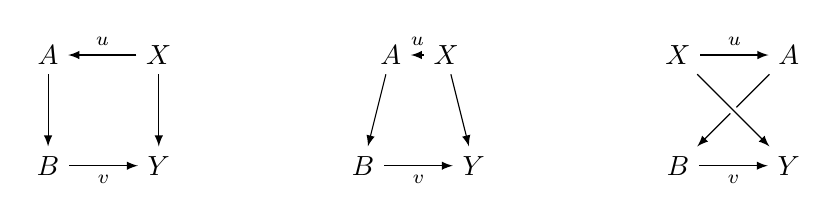
\begin{tikzpicture}[
				x=4em, y=4em,
				dot/.style={
						circle,
						fill=#1,
						inner sep=0pt,
						outer sep=2pt,
						minimum size=4pt,
						draw=none,
					},
				wrap/.style={
						fill=black!5,
						draw=gray,
						rounded corners,
						inner sep=.5em,
					},
			]

			\node (A) at (0,0) {$A$};
			\node (B) at (0,-1) {$B$};
			\node (X) at (1,0) {$X$};
			\node (Y) at (1,-1) {$Y$};
			\draw[-latex] (A) -- (B);
			\draw[-latex] (X) -- (Y);
			\draw[-latex] (B) -- (Y) node[below, pos=.5, font=\scriptsize] {$v$};
			\draw[-latex] (X) -- (A) node[above, pos=.5, font=\scriptsize] {$u$};
			\begin{scope}[xshift=4cm]
				\node (A) at (.25,0) {$A$};
				\node (B) at (0,-1) {$B$};
				\node (X) at (.75,0) {$X$};
				\node (Y) at (1,-1) {$Y$};
				\draw[-latex] (A) -- (B);
				\draw[-latex] (X) -- (Y);
				\draw[-latex] (B) -- (Y) node[below, pos=.5, font=\scriptsize] {$v$};
				\draw[-latex] (X) -- (A) node[above, pos=.5, font=\scriptsize] {$u$};
			\end{scope}
			\begin{scope}[xshift=8cm]
				\node (A) at (1,0) {$A$};
				\node (B) at (0,-1) {$B$};
				\node (X) at (0,0) {$X$};
				\node (Y) at (1,-1) {$Y$};
				\draw[-latex] (A) -- (B);
				\draw[-latex] (B) -- (Y) node[below, pos=.5, font=\scriptsize] {$v$};
				\draw[-latex] (X) -- (A) node[above, pos=.5, font=\scriptsize] {$u$};
				\draw[line width=3pt,white,-] (X) -- (Y);
				\draw[-latex] (X) -- (Y);
			\end{scope}
		\end{tikzpicture}
	\end{center}
	\caption{La ragione dietro la terminologia `freccia ritorta' per la Definizione \ref{def_cat_frecce_ritorte} è che i suoi morfismi si possono pensare come quadrati commutativi dove il dominio orizzontale \(u\) è stato ruotato di mezzo giro.}
\end{figure}
\begin{esercizi}
	\item Sia \(\ctC\) una categoria, \(X\in\ctC_0\) un oggetto, \(f : A\to X\) una freccia: dimostrare che il doppio incubo \((\ctC/X)/f\) è un incubo di \(\ctC\) (su quale oggetto?). Questa `riduzione' di un incubo iterato resta vera per l'incubo della succuba \((A/\ctC)/f\), per \(f/(\ctC/X)\), e per \(f/(A/\ctC)\)?
	\item Un \emph{segmento binario} \((n_0,n_1,t,H)\) consiste di una coppia di interi positivi \(n_0 \le n_1\),con una funzione suriettiva e monotòna \(t : [n_1] \to [n_0]\), e un sottoinsieme \(H\subseteq [n_0]\). Un omomorfismo tra segmenti binari \((n_0,n_1,t,H) \to (n_0',n_1',t',H')\) consiste di una coppia \((f_0,f_1)\) dove
	\begin{itemize}
		\item \(f_1 : [n_1] \to [n_1']\) è una funzione iniettiva e monotòna;
		\item \(f_0 : [n_0] \to [n_0']\) è una funzione monotòna;
		\item il diagramma
		      \[\begin{tikzcd}
				      {[n_1]}\ar[r, "t"]\ar[d, hook, "{f_1}"'] & {[n_0]} \ar[d, "f_0"]\\
				      {[n_1']} \ar[r, "{t'}"'] & {[n_0']}
			      \end{tikzcd}\]
		      è commutativo;
		\item \(f_0^{-1}(H')\subseteq H\).
	\end{itemize}
	Mostrare che questo definisce una categoria \(\cate{Seg}^{[{\circ}{\bullet}]}\) dei segmenti binari.\footnote{Un segmento binario è una rappresentazione discreta e semplificata di un cromosoma: la funzione \(t\) determina una partizione di \([n_1]\) in \(n_0\) sottoinsiemi \(t^{-1}(1),t^{-1}(2),\dots t^{-1}(n_0)\) che si può rappresentare come
	\[[{\circ}{\circ}][{\circ}{\circ}{\circ}{\circ}][{\circ}]\]
	quando \(n_0=3\) e \(n_1=7\); il sottoinsieme \(H\subseteq n_0\) determina poi le regioni del cromosoma \(\chi\) che si vogliono usare nella replicazione, e il suo complementare \(H^c\) quelle che sono silenziate (\emph{masking}). Se ad esempio \(H\subseteq [3]\) è l'insieme \(\{1,3\}\), possiamo colorare la partizione di sopra come
	\[[{\bullet}{\bullet}][{\circ}{\circ}{\circ}{\circ}][{\bullet}].\]
	Invitiamo chi legge a trovare quale possa essere una interpretazione per un omomorfismo di segmenti!}
	\item \'E possibile rappresentare le relazioni (si veda \ref{ex_cat_rels}) sia come spanne che come cospanne. La prima rappresentazione è molto semplice (l'esercizio consiste nel verificare quanto diciamo): una relazione \(R\subseteq A\times B\) corrisponde a una spanna
	\[
		\begin{tikzcd}
			A & R \ar[r, "b"]\ar[l, "a"']& B
		\end{tikzcd}
	\]
	e una spanna dello stesso tipo corrisponde a una relazione non appena la funzione \(R \to A\times B\) che manda \(r\in R\) nella coppia \((a(r),b(r))\) è iniettiva; di converso, la cospanna \(c(R)\) associata alla relazione \(R\) è definita come la categoria che ha per oggetti la somma disgiunta di insiemi \(A+B\), e dove esiste una freccia \(s\to t\) se e solo se \(s\in A,t\in B\) e \((s,t)\in R\). Questa cospanna
	\[
		\begin{tikzcd}
			A \ar[r] & c(R) & \ar[l] B
		\end{tikzcd}
	\]
	si dice il \emph{grafico} di \(R\): per quale motivo? Si disegni la cospanna \(c(R)\) per semplici relazioni tra insiemi finiti; si descriva \(c(R)\) per una relazione \(R\subseteq X\times X\) che sia riflessiva, per una simmetrica, per una transitiva, su un insieme \(X\).
	\item Determinare il giunto di due catene generiche \(\Delta[n] \star \Delta[m]\) come in \ref{ex_cat_catena} e di due cubi \(P[n] \star P[m]\) come in \ref{ex_quadcuboncubo}, e più in generale di due insiemi parzialmente ordinati \(P,Q\). Determinare il giunto di due categorie discrete (prenderle finite!) \(A^\delta \star B^\delta\) come in \ref{ex_cat_discreta} e di due categorie codiscrete \(A^\chi \star B^\chi\): il risultato è ancora codiscreto? Più in generale, determinare il giunto di due gruppi \(\ctG \star \ctG'\) guardati come categorie; il risultato è ancora un gruppo? Determinare il giunto \(\susp(\bbN,+,0) \star \susp(\bbN,+,0)\) del monoide dei numeri naturali con la somma, e \(\susp(\bbN,\max,0) \star \susp(\bbN,\max,0)\) del monoide dove la moltiplicazione è data da \(n\land m \defeq \max\{n,m\}\). C'è una relazione tra \((\ctC\star\ctD)^\op\) e \(\ctD^\op\star\ctC^\op\) (uguali, oposte una dell'altra, nessuna relazione\dots)?
	\item Combinare le costruzioni di prodotto, somma, incubo, succuba, giunto: si può descrivere il giunto \((\ctA\times\ctB)\star\ctC\) in termini di \(\ctA\star\ctC\), \(\ctB\star\ctC\)? Come descrivere \((\ctC+\ctD)/X\) al variare di \(X\in(\ctC+\ctD)_0\)? Come descrivere \((\ctA/A)\star(\ctB/B)\), \((A/\ctA)\star(B/\ctB)\), \((\ctA/A)\star(B/\ctB)\)? Come descrivere \((\ctA\star\ctB)+\ctC\)?
\end{esercizi}
